\documentclass[a4j,dvipdfmx]{jarticle}
%----------------------------------------------------------------------
\usepackage{graphicx}
%\usepackage{amsmath}
%\usepackage{amssymb}
%\usepackage{bm}
%\usepackage{fancybox}
\usepackage{fancyhdr}
\usepackage{lastpage}
%\usepackage{color}
\usepackage{multicol}
\usepackage{listings,jlisting}
\usepackage{ascmac}
%----------------------------------------------------------------------
%\setlength{\topmargin}{-0.5in}
%\addtolength{\headheight}{1cm}
%%\setlength{\headsep}{0mm}
%\setlength{\oddsidemargin}{-0.5in}
%%\setlength{\evensidemargin}{-0.5in}
%\addtolength{\textwidth}{1.5in}
%\addtolength{\textheight}{1in}
%----------------------------------------------------------------------
%\setlength{\columnsep}{2zw}
%\setlength{\columnseprule}{0.4pt}
%----------------------------------------------------------------------
\pagestyle{fancy}
\lhead{2016/07/19}
\rhead{配布資料(\thepage / \pageref{LastPage})}
\cfoot{}
\chead{\textgt{システムプログラミング2 第13回}}
%----------------------------------------------------------------------
\begin{document}
\def\lstlistingname{リスト}
\lstset{language=C,
  numbers=left,
  basicstyle={\small\ttfamily},
  columns=[l]{fullflexible},
  keepspaces=true,
  frame=shadowbox,
  commentstyle=\slshape
}
%----------------------------------------------------------------------

%\begin{figure}[hbtp]
%\begin{center}
%\includegraphics[height=2.5cm]{state.pdf}
%\caption{単語の長さをカウントするアルゴリズム}
%\end{center}
%\end{figure}

今回は、プログラムで他のプログラムを起動する方法を学ぶ。

\begin{enumerate}
\item Fork-Exec 方式

UNIXで新しくプログラム起動するために用いられてきた方式のことである。
fork(プロセスの生成)とexec(プログラムロード・実行)の2段階で目的を達成する。

\begin{enumerate}
\item fork

\verb/fork/システムコールを用い、新しいプロセスを作成する。

\begin{lstlisting}[numbers=none]
書式: #include <unistd.h>
       int fork(void);

解説: プロセスのコピーを作る。親プロセスには子プロセスのPIDが返される。
       エラー時はが返される。
\end{lstlisting}

\verb/fork/システムコールを実行した「プロセスがコピーされ」る。
元のプロセスを{\bf 親プロセス}、
コピーして作ったプロセスを{\bf 子プロセス}と呼ぶ。
図\ref{fig1}にforkの様子を、
リスト\ref{list1}に\verb/fork/システムコールを実行するプログラムの例を、
以下にforkの処理手順を示す。

\begin{enumerate}
\item 親プロセスがプログラム実行中に\verb/fork/システムコールを実行する。
\item 新しいプロセス(子プロセス)が作られ、親プロセスの内容がコピーされる。
\item 子プロセスには、
メモリ空間(プログラム、変数(データ)、スタック)、
プロセスの状態(どのファイルをオープン中か、シグナルハンドラの登録等)、
CPUの状態(CPUレジスタの値、SPの値、PCの値、フラグの値)等、
全ての情報がコピーされる。
ただし、プロセス番号(PID:Process ID)値は親子プロセスで異なる。
\item 親プロセスは\verb/fork/システムコールを終了しプログラムの実行を再開する。
この時、\verb/fork/システムコールは子プロセスのPIDを返す。
\item 子プロセスは\verb/fork/システムコールを呼出した瞬間のコピーなので、
\verb/fork/システムコールが終了するところからプログラム実行を開始する。
この時、\verb/fork/システムコールは\verb/0/を返す。
\end{enumerate}

\begin{figure}[hbtp]
\begin{center}
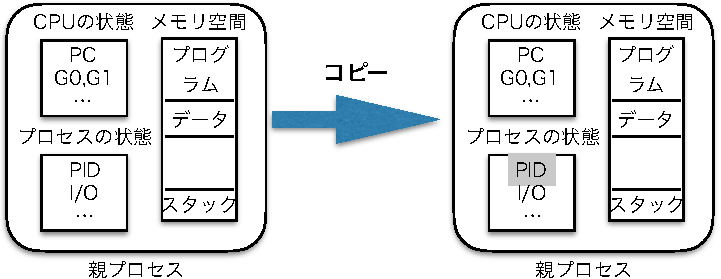
\includegraphics[scale=0.8]{fork-crop.pdf}
\caption{forkの仕組み}
\label{fig1}
\end{center}
\end{figure}

\lstinputlisting[label=list1, caption=forkの使用例]{forktest.c}

\end{enumerate}
\end{enumerate}
\end{document}
